\documentclass[aspectratio=169, xcolor={dvipsnames}]{beamer}

\usepackage{tikz}
\usetikzlibrary{shapes.geometric, arrows.meta, positioning, calc, backgrounds, fit}
\usepackage{graphicx}
\usepackage{booktabs}

% Colors based on user prompt
\definecolor{DarkNavy}{RGB}{20, 40, 80}
\definecolor{LightNavy}{RGB}{35, 60, 110}
\definecolor{PaleBlue}{RGB}{230, 240, 250}
\definecolor{MutedTeal}{RGB}{50, 140, 140}
\definecolor{White}{RGB}{255, 255, 255}

% Beamer Theme Customization
\usetheme{Madrid}

% Apply the color theme
\setbeamercolor{structure}{fg=DarkNavy}
\setbeamercolor{palette primary}{bg=DarkNavy,fg=white}
\setbeamercolor{palette secondary}{bg=LightNavy,fg=white}
\setbeamercolor{palette tertiary}{bg=DarkNavy,fg=white}
\setbeamercolor{palette quaternary}{bg=DarkNavy,fg=white}
\setbeamercolor{title}{bg=DarkNavy,fg=white}
\setbeamercolor{item projected}{bg=DarkNavy,fg=white}

% Customize the footline
\setbeamertemplate{footline}
{
  \leavevmode%
  \hbox{%
  \begin{beamercolorbox}[wd=.5\paperwidth,ht=2.25ex,dp=1ex,center]{author in head/foot}%
    \usebeamerfont{author in head/foot}\insertshortauthor
  \end{beamercolorbox}%
  \begin{beamercolorbox}[wd=.5\paperwidth,ht=2.25ex,dp=1ex,center]{title in head/foot}%
    \usebeamerfont{title in head/foot}\insertshorttitle
  \end{beamercolorbox}}%
  \vskip0pt%
}

% Make itemize bullets spheres
\setbeamertemplate{itemize items}[sphere]
\setbeamertemplate{itemize subitem}[sphere]

\title[CodeGraph: Repository-Level Structural Retrieval]{CodeGraph: Repository-Level Structural Retrieval\\for AI Coding Agents via Personalized PageRank}
\author[Alexandru Toma]{Alexandru Toma}
\institute[]{
  Babeș - Bolyai University \\ 
  Faculty of Mathematics and Computer Science \\
  \vspace{0.3cm}
  SCSS Conference 2026
}
\date{}

\begin{document}

% Slide 1
\begin{frame}
    \titlepage
\end{frame}

% Slide 2: Ambiguity of Natural Language
\begin{frame}{The Ambiguity of Natural Language in Agentic Coding}
    \begin{itemize}
        \item \textbf{The Mismatch:} Developers describe bugs abstractly (e.g., "fix permissions logic").
        \item \textbf{The Target:} The relevant file often has a specific identifier (e.g., \texttt{global\_settings.py}).
        \item \textbf{The Result:} Because of this vocabulary gap, pure text similarity often misses the exact implementation location.
    \end{itemize}
    \vspace{0.3cm}
    \begin{center}
    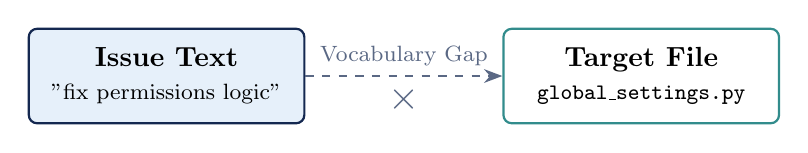
\begin{tikzpicture}[
        node distance=0.8cm and 1.5cm,
        doc/.style={draw=DarkNavy, thick, fill=PaleBlue, minimum width=3.5cm, minimum height=1.2cm, align=center, rounded corners=3pt},
        code/.style={draw=MutedTeal, thick, fill=white, minimum width=3.5cm, minimum height=1.2cm, align=center, rounded corners=3pt},
        arrow/.style={-Stealth, thick, DarkNavy!70, dashed}
    ]
        \node[doc] (prompt) {\textbf{Issue Text}\\ \footnotesize "fix permissions logic"};
        \node[code, right=2.5cm of prompt] (file) {\textbf{Target File}\\ \footnotesize \texttt{global\_settings.py}};
        
        \draw[arrow] (prompt) -- node[above, font=\footnotesize] {Vocabulary Gap} node[below, font=\Large] {$\times$} (file);
    \end{tikzpicture}
    \end{center}
\end{frame}

% Slide 3: Code is a Graph, Not Flat Text
\begin{frame}{Code is a Graph, Not Flat Text}
    \begin{itemize}
        \item \textbf{Code is not just text.} A repository is a structured network of files, classes, and methods.
        \item \textbf{Explicit Syntax:} Components are connected by explicit relationships (e.g., imports, calls).
        \item \textbf{The Intuition:} Let relevance travel through these structural relationships, not just through token overlap.
    \end{itemize}
    \vspace{0.3cm}
    \begin{center}
    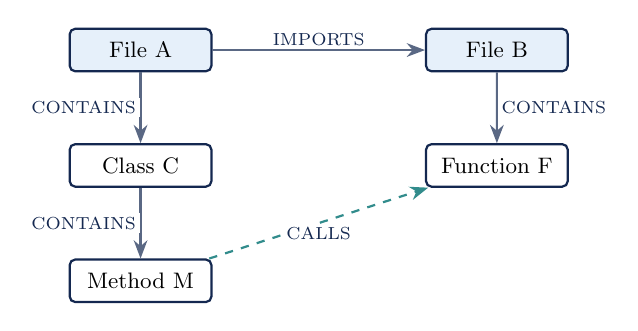
\begin{tikzpicture}[
        node distance=1.5cm, auto, scale=0.9, transform shape,
        entity/.style={draw=DarkNavy, thick, fill=white, minimum width=2cm, minimum height=0.6cm, align=center, font=\small, rounded corners=2pt},
        edge/.style={-Stealth, DarkNavy!70, thick},
        lbl/.style={font=\scriptsize, text=DarkNavy, fill=white, inner sep=1.5pt}
    ]
        \node[entity, fill=PaleBlue] (f1) {File A};
        \node[entity, fill=PaleBlue, right=3cm of f1] (f2) {File B};
        \draw[edge] (f1) -- node[lbl] {IMPORTS} (f2);
        
        \node[entity, below=1cm of f1] (c1) {Class C};
        \node[entity, below=1cm of f2] (func) {Function F};
        \draw[edge] (f1) -- node[lbl, left] {CONTAINS} (c1);
        \draw[edge] (f2) -- node[lbl, right] {CONTAINS} (func);
        
        \node[entity, below=1cm of c1] (m1) {Method M};
        \draw[edge] (c1) -- node[lbl, left] {CONTAINS} (m1);
        \draw[edge, dashed, MutedTeal] (m1) -- node[lbl, below] {CALLS} (func);
    \end{tikzpicture}
    \end{center}
\end{frame}

% Slide 4a: Indexing Phase
\begin{frame}{System Architecture - Indexing Phase (Overview)}
    \begin{itemize}
        \item Raw source code is transformed into a persistent graph in Neo4j.
        \item Happens \textbf{once} before any retrieval queries.
        \item Replaces fragile text indexes and makes the runtime stage fast and stable.
    \end{itemize}
    \vspace{0.8cm}
    \begin{center}
    
\begin{tikzpicture}[node distance=3cm, auto, scale=0.9, transform shape]
        \node[draw=DarkNavy, thick, rounded corners, fill=PaleBlue, text width=2cm, align=center, minimum height=1cm] (src) {Source Code};
        \node[draw=DarkNavy, thick, rounded corners, fill=LightNavy, text=White, right of=src, text width=2.5cm, align=center, minimum height=1cm] (ts) {Tree-sitter};
        \node[draw=DarkNavy, thick, rounded corners, fill=MutedTeal, text=White, right of=ts, text width=2cm, align=center, minimum height=1cm] (ast) {AST};
        \node[draw=DarkNavy, thick, rounded corners, fill=DarkNavy, text=White, right of=ast, text width=2cm, align=center, minimum height=1cm] (neo) {Neo4j Graph};
        \draw[->, thick, DarkNavy] (src) -- (ts);
        \draw[->, thick, DarkNavy] (ts) -- (ast);
        \draw[->, thick, DarkNavy] (ast) -- (neo);
    \end{tikzpicture}
    \end{center}
\end{frame}

% Slide 4b: 4-Entity Model
\begin{frame}{The 4-Entity Model \& Graph Construction}
    \begin{itemize}
        \item \textbf{Coarse-Grained Abstraction:} We extract only four entity types (Files, Classes, Functions, Methods).
        \item \textbf{Explicit Syntactic Edges:} \texttt{IMPORTS}, \texttt{CALLS}, \texttt{CONTAINS}, \texttt{INHERITS\_FROM}.
        \item \textbf{Crucial Choice:} We avoid full AST-level density and file-proximity heuristics because overly dense representations dilute the relevance signal.
    \end{itemize}
    \vspace{0.5cm}
    \begin{center}
        \textit{(A precise structure optimized for algorithmic traversal)}
    \end{center}
\end{frame}

% Slide 5a: Retrieval Phase
\begin{frame}{System Architecture - Retrieval Phase (Overview)}
    \begin{itemize}
        \item \textbf{No LLMs in the retrieval loop.}
        \item Lexical matching extracts seed nodes from the issue description.
        \item Global ranking is computed purely via Personalized PageRank (PPR).
        \item The retrieval loop remains deterministic, low-latency, and reproducible.
    \end{itemize}
    \vspace{0.8cm}
    \begin{center}
    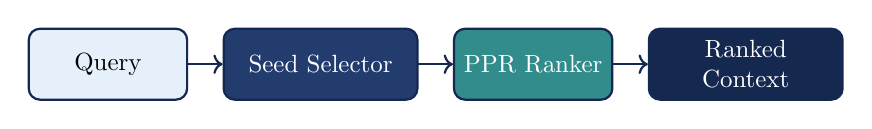
\begin{tikzpicture}[node distance=3cm, auto, scale=0.9, transform shape]
        \node[draw=DarkNavy, thick, rounded corners, fill=PaleBlue, text width=2cm, align=center, minimum height=1cm] (query) {Query};
        \node[draw=DarkNavy, thick, rounded corners, fill=LightNavy, text=White, right of=query, text width=2.5cm, align=center, minimum height=1cm] (seeds) {Seed Selector};
        \node[draw=DarkNavy, thick, rounded corners, fill=MutedTeal, text=White, right of=seeds, text width=2cm, align=center, minimum height=1cm] (ppr) {PPR Ranker};
        \node[draw=DarkNavy, thick, rounded corners, fill=DarkNavy, text=White, right of=ppr, text width=2.5cm, align=center, minimum height=1cm] (ctx) {Ranked Context};
        \draw[->, thick, DarkNavy] (query) -- (seeds);
        \draw[->, thick, DarkNavy] (seeds) -- (ppr);
        \draw[->, thick, DarkNavy] (ppr) -- (ctx);
    \end{tikzpicture}
    \end{center}
\end{frame}

% Slide 5b: Walkthrough
\begin{frame}{Walkthrough - The Anatomy of a Query}
    \begin{enumerate}
        \item \textbf{Query:} e.g., "fix SQL compilation"
        \item \textbf{Seeds:} Map lexical terms to graph entry points (e.g., \texttt{SQLCompiler}).
        \item \textbf{Propagation:} Personalized PageRank diffuses relevance structurally.
        \item \textbf{Penalization:} Generic hubs (like loggers) are downgraded.
        \item \textbf{Context:} Subgraph collapses into a ranked payload.
    \end{enumerate}
    \vspace{0.5cm}
    \begin{center}
        \large \textbf{\textcolor{MutedTeal}{A deterministic traversal from lexical match to structural relevance.}}
    \end{center}
\end{frame}

% Slide 6: Evaluation
\begin{frame}{Evaluation Setup (SWE-bench Lite)}
    \begin{itemize}
        \item \textbf{Dataset:} 300 real-world GitHub issues from 12 Python repositories.
        \item \textbf{The Task:} Given only the natural-language issue, accurately rank the file that the human developer eventually patched.
        \item \textbf{Constraint:} Evaluated under a fixed context budget, exactly mirroring how agents operate.
    \end{itemize}
    \vspace{0.5cm}
    \begin{center}
        
\begin{tikzpicture}[
            scale=0.9, transform shape,
            box/.style={draw=DarkNavy, thick, fill=white, minimum width=3cm, minimum height=1.5cm, align=center, font=\small},
            arrow/.style={-Stealth, thick, MutedTeal}
        ]
            \node[box] (issue) {\textbf{GitHub Issue}\\ \vspace{0.1cm} \textit{Natural Language}};
            \node[box, right=1.5cm of issue, fill=PaleBlue] (retriever) {Retriever};
            \node[box, right=1.5cm of retriever, align=left] (files) {\textbf{Ranked Files}\\ \textcolor{MutedTeal}{\#1 Patched File}\\ \#2 Other File\\ ...};
            
            \draw[arrow] (issue) -- (retriever);
            \draw[arrow] (retriever) -- (files);
        \end{tikzpicture}
    \end{center}
\end{frame}

% Slide 7: Quantitative Results
\begin{frame}{Quantitative Results}
    \textbf{Graph propagation provides a substantial improvement over text-only retrieval.}
    \vspace{0.8cm}
    \begin{center}
    \begin{tabular}{lcc}
        \toprule
        \textbf{Method} & \textbf{Recall@10} & \textbf{Recall@30} \\
        \midrule
        BM25 (Text Baseline) & 58.0\% & 69.3\% \\
        CodeGraph (Uniform PPR) & \textbf{\textcolor{MutedTeal}{74.0\%}} & \textbf{\textcolor{MutedTeal}{83.0\%}} \\
        \bottomrule
    \end{tabular}
    \end{center}
\end{frame}

% Slide 8: Reachability
\begin{frame}{The Reachability Bottleneck}
    \begin{itemize}
        \item \textbf{The True Ceiling:} Seed reachability limits retrieval success.
        \item If seeds hit the right structural neighborhood, the ranking succeeds.
        \item If seeds completely miss, no ranking method can recover the file.
        \item \textbf{Result:} Remaining failures split cleanly into structural gaps and lexical gaps.
    \end{itemize}
    \vspace{0.5cm}
    \begin{center}
    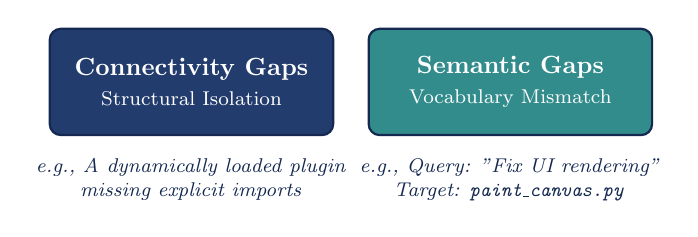
\begin{tikzpicture}[
        scale=0.9, transform shape,
        box/.style={text=White, thick, rounded corners, minimum width=4cm, minimum height=1.5cm, align=center},
        ex/.style={font=\footnotesize, text=DarkNavy, align=center}
    ]
        \node[box, fill=LightNavy, draw=DarkNavy] (conn) at (0,0) {\textbf{Connectivity Gaps}\\ \footnotesize Structural Isolation};
        \node[box, fill=MutedTeal, draw=DarkNavy] (sem) at (4.5,0) {\textbf{Semantic Gaps}\\ \footnotesize Vocabulary Mismatch};
        
        \node[ex, below=0.2cm of conn] {\textit{e.g., A dynamically loaded plugin}\\\textit{missing explicit imports}};
        \node[ex, below=0.2cm of sem] {\textit{e.g., Query: "Fix UI rendering"}\\\textit{Target: \texttt{paint\_canvas.py}}};
    \end{tikzpicture}
    \end{center}
\end{frame}

% Slide 9a: Ecosystem
\begin{frame}{The CodeGraph Ecosystem}
    \textbf{A fully realized toolset, not just an abstract experiment.}
    \vspace{0.5cm}
    \begin{itemize}
        \item \textbf{MCP Server:} Enables autonomous agents via standard tools:
        \begin{itemize}
            \item \texttt{get\_relevant\_context}
            \item \texttt{query\_dependencies}
        \end{itemize}
        \vspace{0.2cm}
        \item \textbf{CLI:} Fast repository querying for developers:
        \begin{itemize}
            \item \texttt{codegraph index} \textbar\ \texttt{codegraph clone} \textbar\ \texttt{codegraph query}
        \end{itemize}
        \vspace{0.2cm}
        \item \textbf{Web Visualizer:} A structural debugging interface for observing seed propagation.
    \end{itemize}
\end{frame}

% Slide 9b: Visualizer
\begin{frame}{The Web Visualizer in Action}
    \begin{itemize}
        \item \textbf{Observable Graph:} Turns the "black box" of retrieval into an observable structure.
        \item \textbf{Debugging:} Visually inspect seeds, trace connectivity breaks, and understand the precise flow of Personalized PageRank relevance.
    \end{itemize}
    \vspace{0.2cm}
    \begin{center}
        
\includegraphics[width=0.8\textwidth]{../../assets/visualizer_query_results.png}
    \end{center}
\end{frame}

% Slide 10: Conclusion
\begin{frame}{Conclusion \& Future Work}
    \textbf{To wrap up:}
    \begin{itemize}
        \item \textbf{Result:} Code structure improves context retrieval beyond pure text similarity.
        \item \textbf{Value:} Deterministic, reproducible retrieval for coding agents.
        \item \textbf{Ceiling:} Seed reachability is the primary bottleneck.
    \end{itemize}
    \vspace{0.5cm}
    \textbf{Future Work:}
    \begin{itemize}
        \item Extending architectural support to Java, TypeScript, and Spring Boot.
        \item Improving seed selection methods to address vocabulary mismatch.
    \end{itemize}
\end{frame}

% Slide 11: QA
\begin{frame}[plain]
    \begin{center}
        \vspace{1cm}
        {\Huge \textbf{Thank You}} \\
        \vspace{1cm}
        \Large Alexandru Toma \\
        \large Babeș-Bolyai University \\
        \vspace{1cm}
        \textbf{\textcolor{MutedTeal}{Questions?}}
    \end{center}
\end{frame}

\end{document}
